\documentclass[sigconf,nonacm]{acmart}

\usepackage{booktabs}
\usepackage{amsfonts}
\usepackage{amsmath}
%% amssymb omitted: acmart already loads it; duplicate causes \Bbbk clash
\usepackage{nicefrac}
\usepackage{graphicx}
\usepackage{subcaption}
\usepackage{multirow}
\usepackage{xcolor}
\usepackage{microtype}
\usepackage{tikz}
\usetikzlibrary{shapes.geometric, arrows.meta, positioning, fit, backgrounds}
\tolerance=1000
\emergencystretch=1em

%%% Remove ACM copyright/DOI for submission
\settopmatter{printacmref=false}
\renewcommand\footnotetextcopyrightpermission[1]{}
\pagestyle{plain}

\begin{document}

\title{When Does Conformer Geometry Help? Complementarity of 3D Ensemble Statistics and 2D Fingerprints for Molecular Property Prediction}

\author{Anonymous Authors}
\affiliation{%
  \institution{Under Review}
  \country{}
}

\begin{abstract}
We study when three-dimensional conformer ensemble statistics complement two-dimensional molecular fingerprints for property prediction. Using Distribution Kernel Operators (DKOs), we extract mean and covariance features from conformer ensembles and evaluate 13 architectures across 8+ datasets. Morgan fingerprints with XGBoost outperform all neural conformer methods on every benchmark. However, hybrid features combining fingerprints with conformer statistics yield 9.9\% RMSE reduction on ESOL, 3.9\% on FreeSolv, and 4.2\% on QM9-HOMO---establishing conformer statistics as complementary descriptors for solvation-dependent properties. This complementarity is selective: a property taxonomy (solvation vs.\ steric vs.\ electronic) predicts when conformer features add value. Mechanistic analysis via mutual information reveals that conformer features encode orthogonal geometric signal (surface area, shape) absent from fingerprints. Among neural architectures, learned gating for mean/covariance fusion significantly outperforms attention ($p < 0.001$), and five simple covariance summary statistics outperform complex representations.
\end{abstract}

\begin{CCSXML}
<ccs2012>
<concept>
<concept_id>10010147.10010178</concept_id>
<concept_desc>Computing methodologies~Machine learning</concept_desc>
<concept_significance>500</concept_significance>
</concept>
<concept>
<concept_id>10010147.10010257</concept_id>
<concept_desc>Computing methodologies~Modeling and simulation</concept_desc>
<concept_significance>300</concept_significance>
</concept>
<concept>
<concept_id>10003120.10003130</concept_id>
<concept_desc>Human-centered computing~Collaborative and social computing</concept_desc>
<concept_significance>100</concept_significance>
</concept>
</ccs2012>
\end{CCSXML}

\ccsdesc[500]{Computing methodologies~Machine learning}
\ccsdesc[300]{Computing methodologies~Modeling and simulation}
\ccsdesc[100]{Applied computing~Computational biology}

\keywords{molecular property prediction, conformer ensembles, distribution kernel operators, fingerprints, 3D descriptors, covariance representations}

\maketitle

%──────────────────────────────────────────────────────────────
\section{Introduction}
%──────────────────────────────────────────────────────────────

Molecular property prediction is a cornerstone of computational chemistry and drug discovery. While graph neural networks (GNNs) operating on 2D molecular graphs have achieved remarkable success~\cite{gilmer2017mpnn,yang2019chemprop}, a molecule's biological activity fundamentally depends on its three-dimensional geometry. Small molecules adopt multiple low-energy conformations in solution, and properties such as solvation free energy and lipophilicity are Boltzmann-weighted averages over this conformational ensemble~\cite{hawkins2017conformation}.

This has motivated a growing body of work on conformer ensemble methods~\cite{axelrod2024marcel,ganea2021geomol,stark2022equivariant} and 3D-aware GNNs~\cite{schutt2017schnet,gasteiger2020dimenet,schutt2021painn}, which incorporate 3D geometry for property prediction. However, a fundamental question remains: \emph{when does explicit 3D conformer geometry provide signal beyond what 2D molecular descriptors already capture?}

We address this question through a systematic benchmark of 13 model architectures across 8+ datasets. Our approach extracts first-order (mean $\boldsymbol{\mu}$) and second-order (covariance $\boldsymbol{\Sigma}$) statistics from conformer features and evaluates multiple fusion architectures.
\textbf{Scope:} this study focuses on regression tasks; preliminary experiments on classification (BACE, BBBP) showed degenerate DKO behavior, suggesting architectural adaptation is needed for discrete outputs.
Our key contributions are:

\begin{enumerate}
    \item \textbf{DKO framework}: A Distribution Kernel Operator architecture with explicit $\boldsymbol{\mu}$/$\boldsymbol{\Sigma}$ modeling, 7 covariance representation variants, and 28 enhanced 3D shape descriptors, including a gated fusion mechanism that significantly outperforms attention ($p < 0.001$).
    \item \textbf{Comprehensive benchmark}: 13 model architectures evaluated across 6 MoleculeNet regression datasets, 4 Kraken steric descriptors, BDE, and Drugs-75K, with 10-seed statistical validation.
    \item \textbf{Complementarity finding}: While fingerprints alone beat all neural conformer methods, hybrid features improve predictions on solvation-related tasks by up to $9.9\%$---establishing conformer statistics as complementary, not competing, descriptors.
    \item \textbf{Mechanistic understanding}: Information-theoretic analysis reveals \emph{why} fingerprints dominate and \emph{why} hybrids help. A property taxonomy (solvation vs.\ steric vs.\ electronic) predicts when conformer features add value (Figure~\ref{fig:taxonomy}).
\end{enumerate}

%──────────────────────────────────────────────────────────────
\section{Related Work}
%──────────────────────────────────────────────────────────────

\textbf{Conformer ensemble methods.}
The MARCEL benchmark~\cite{axelrod2024marcel} established standardized evaluation for conformer ensemble learning on Kraken steric descriptors, bond dissociation energies, and electronic properties. GeoMol~\cite{ganea2021geomol} generates conformers via end-to-end learning, while 3D Infomax~\cite{stark2022equivariant} uses contrastive 3D pre-training to enrich 2D representations. These approaches typically aggregate conformer features via mean pooling or attention, discarding distributional information.

\textbf{3D molecular representations.}
SchNet~\cite{schutt2017schnet} introduced continuous-filter convolutions for modeling quantum interactions from 3D coordinates. DimeNet~\cite{gasteiger2020dimenet} and its successor DimeNet++~\cite{gasteiger2021dimenetpp} incorporate directional message passing using bond angles. PaiNN~\cite{schutt2021painn} achieves equivariant message passing for tensorial properties. SphereNet~\cite{liu2022spherical} extends to spherical coordinates, while GemNet~\cite{klicpera2020gemnet} uses geometric message passing with universal approximation guarantees. Uni-Mol~\cite{zhou2023unimol} provides large-scale 3D pre-training, and TorchMD-NET~\cite{tholke2022torchmdnet} combines equivariant transformers with molecular dynamics potentials. These methods operate on single conformers or equilibrium geometries; our work instead models the \emph{ensemble distribution} via summary statistics.

\textbf{Molecular fingerprints and classical ML.}
Extended-connectivity fingerprints~\cite{rogers2010ecfp} remain the dominant representation in cheminformatics.
Combined with gradient-boosted trees~\cite{chen2016xgboost}, they provide baselines that neural methods frequently fail to surpass~\cite{wu2018moleculenet}.
Our work quantifies this gap and identifies where conformer features add complementary value.

\textbf{Set aggregation architectures.}
Processing unordered conformer sets requires permutation-invariant architectures.
DeepSets~\cite{zaheer2017deepsets} provides the theoretical foundation, while Set Transformer~\cite{lee2019set} introduces attention-based aggregation.
We compare these against our DKO framework, which models the distribution's first and second moments explicitly.

\textbf{Kernel methods in molecular ML.}
Kernel methods have a long history in molecular property prediction~\cite{rupp2012randomml}. Our DKO builds on distributional kernels that compare molecules via their conformer distributions, using a learned positive semi-definite kernel $\mathbf{K} = \mathbf{L}\mathbf{L}^\top$.

%──────────────────────────────────────────────────────────────
\section{Methods}
%──────────────────────────────────────────────────────────────

\begin{figure*}[t]
\centering
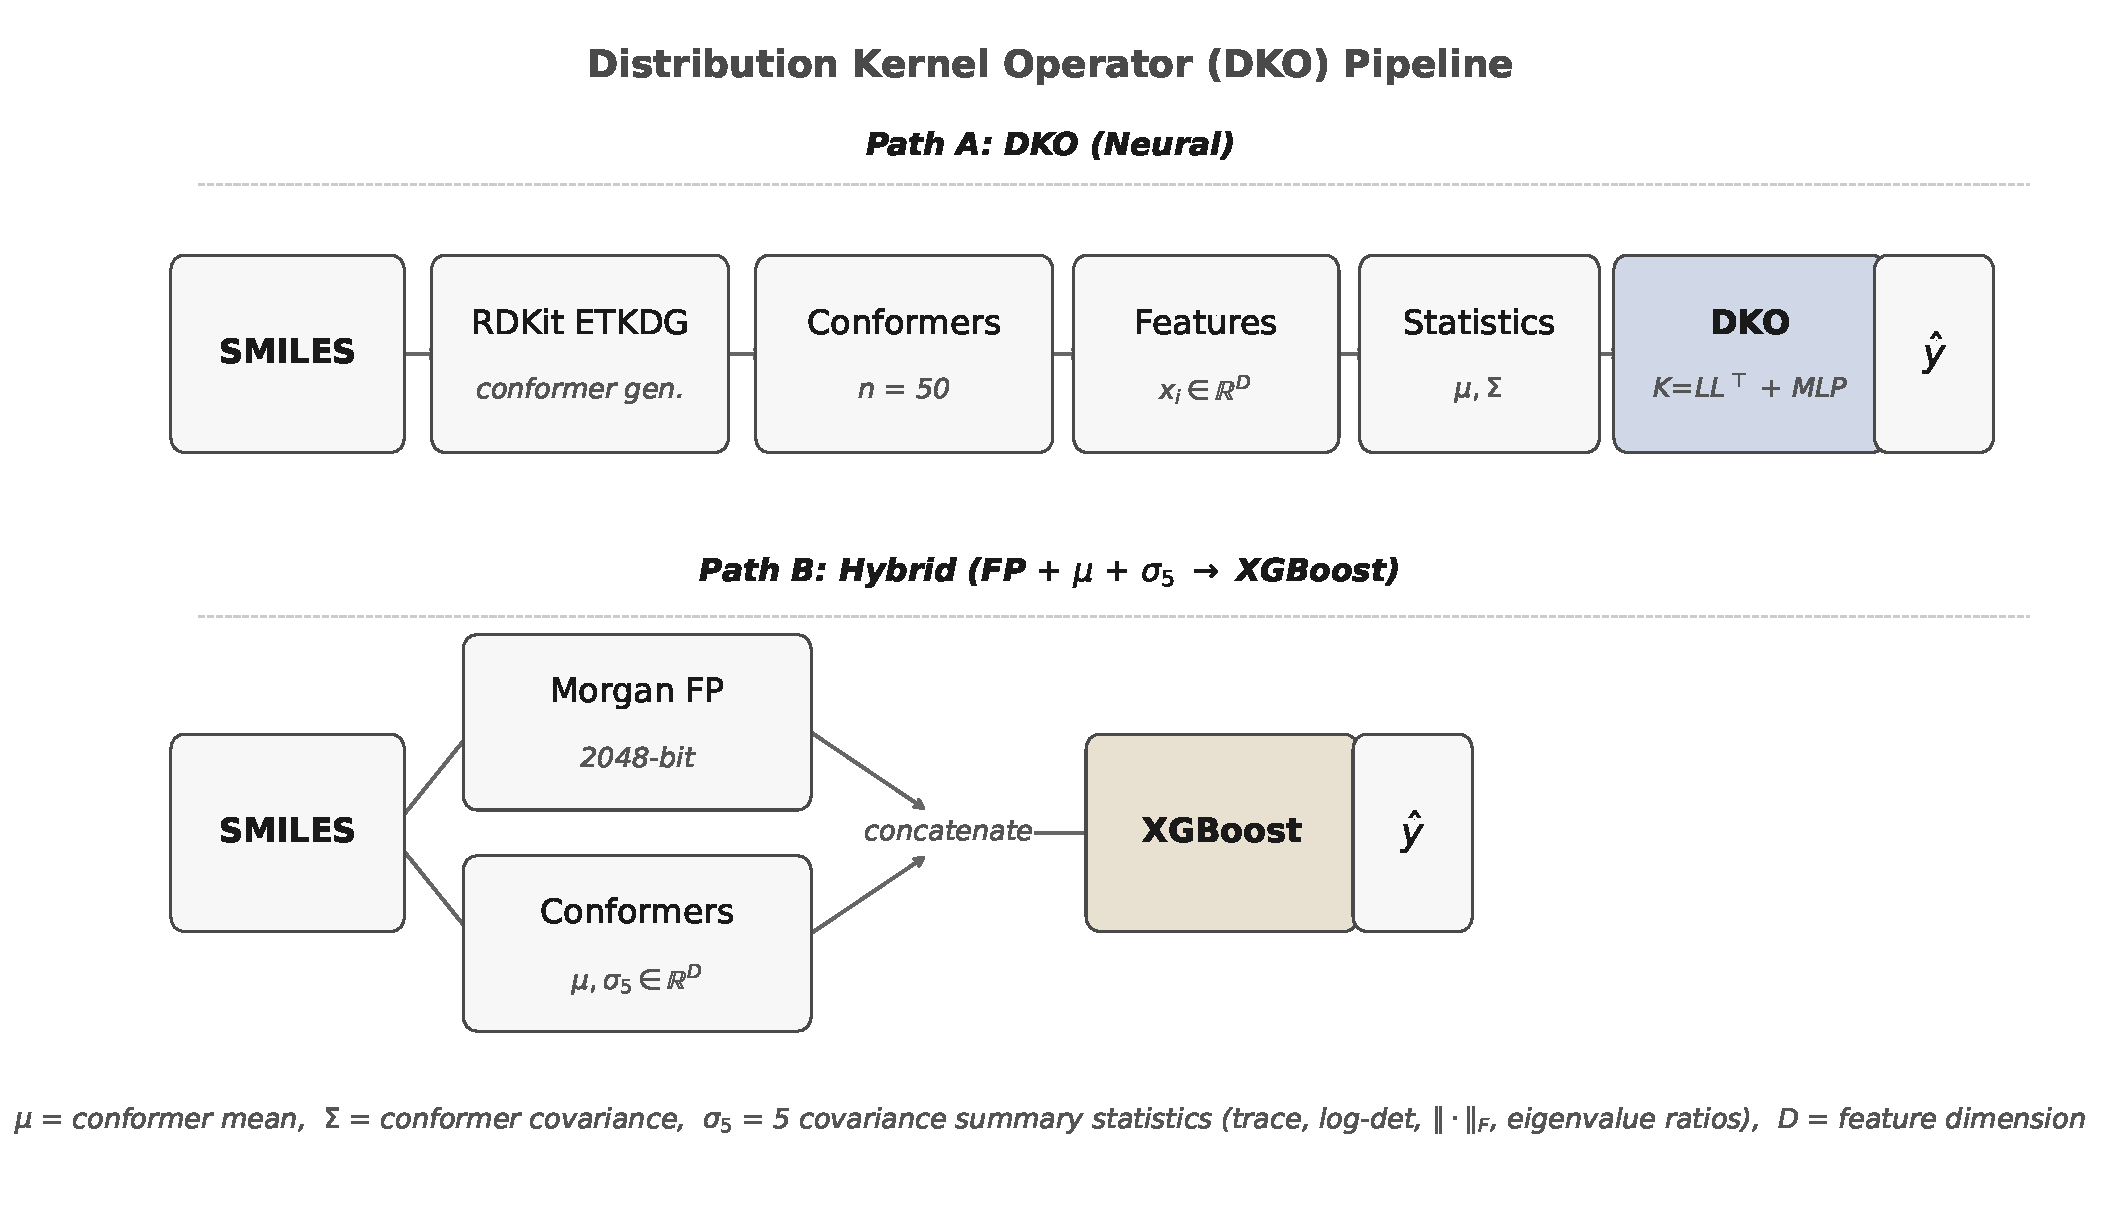
\includegraphics[width=0.95\textwidth]{figures/fig_architecture.pdf}
\caption{Overview of the DKO pipeline. \textbf{Left}: Conformer generation and feature extraction. Each molecule's SMILES is converted to $n{=}50$ 3D conformers via ETKDG; per-conformer geometric features (distances, angles, torsions within 4\AA{} cutoff, plus 19-dim atom features) are computed and padded/truncated to $D{=}1024$. \textbf{Center}: DKO architecture. Ensemble mean $\boldsymbol{\mu}$ and covariance $\boldsymbol{\Sigma}$ are extracted; a low-rank kernel $\mathbf{K}{=}\mathbf{L}\mathbf{L}^\top$ transforms these into predictions via variant-specific fusion (gated, invariants, etc.). \textbf{Right}: Hybrid approach. Morgan fingerprints (2048-bit) are concatenated with $\boldsymbol{\mu}$ and 5 covariance summary statistics, then fed to XGBoost.}
\label{fig:arch}
\end{figure*}

Figure~\ref{fig:arch} provides an overview of the DKO pipeline and hybrid approach.

\subsection{Conformer Generation and Feature Extraction}

For each molecule, we generate $n = 50$ conformers using RDKit's ETKDG (Experimental Torsion-angle preference with Knowledge and Distance Geometry) algorithm~\cite{riniker2015etkdg} with energy minimization via the MMFF94 (Merck Molecular Force Field) force field.
The choice of $n{=}50$ follows the MARCEL benchmark protocol~\cite{axelrod2024marcel}; ablating this hyperparameter is left to future work.

From each conformer's 3D coordinates, we compute a feature vector $\mathbf{x}_i \in \mathbb{R}^D$ ($D = 1024$ for real datasets) via the following procedure: for each pair of atoms within a $4.0$\AA{} cutoff, we compute the interatomic distance; for each bonded triple, the bond angle; and for each bonded quadruple, the torsion angle (encoded as $\cos\theta, \sin\theta$). These geometric features are concatenated with 19-dimensional per-atom features (element type, hybridization, formal charge, etc.) and zero-padded or truncated to a fixed dimension $D$.

Given a conformer ensemble $\{\mathbf{x}_1, \ldots, \mathbf{x}_n\}$, we compute:
\begin{align}
    \boldsymbol{\mu} &= \frac{1}{n}\sum_{i=1}^{n} \mathbf{x}_i \in \mathbb{R}^D, \label{eq:mu} \\
    \boldsymbol{\Sigma} &= \frac{1}{n-1}\sum_{i=1}^{n}(\mathbf{x}_i - \boldsymbol{\mu})(\mathbf{x}_i - \boldsymbol{\mu})^\top + \lambda\mathbf{I} \in \mathbb{R}^{D \times D}, \label{eq:sigma}
\end{align}
where $\lambda = 10^{-2}$ provides regularization against near-singular covariance matrices.

\subsection{DKO Architecture}

The Distribution Kernel Operator (DKO) maps the pair $(\boldsymbol{\mu}, \boldsymbol{\Sigma})$ to a molecular property prediction. The core architecture consists of:

\textbf{Kernel construction.} We parameterize a positive semi-definite kernel via a low-rank factorization $\mathbf{K} = \mathbf{L}\mathbf{L}^\top$, where $\mathbf{L} \in \mathbb{R}^{k \times D}$ is a learnable projection with output dimension $k = 64 \ll D$.

\textbf{Branch prediction network.} A multi-layer perceptron processes the kernel-transformed features to produce scalar predictions, combining the first-order signal from $\boldsymbol{\mu}$ with second-order signal from $\boldsymbol{\Sigma}$.

\subsection{DKO Variants}

We evaluate 7 covariance representation strategies, all using eigendecomposition of $\boldsymbol{\Sigma}$ (with a diagonal proxy when $D > 256$):

\begin{itemize}
    \item \textbf{dko\_gated}: Learned sigmoid gate fusing separate $\boldsymbol{\mu}$ and $\boldsymbol{\Sigma}$ prediction streams.
    \item \textbf{dko\_invariants}: 5 summary statistics from $\boldsymbol{\Sigma}$: trace, log-determinant, Frobenius norm, top eigenvalue ratio, and spectral ratio $\lambda_1/\lambda_k$. Note that trace and Frobenius norm are not independent ($\mathrm{tr} = \sum\lambda_i$, $\|\cdot\|_F^2 = \sum\lambda_i^2$); we retain both as they provide complementary scale vs.\ spread information.
    \item \textbf{dko\_eigenspectrum}: Top-$k$ eigenvalues concatenated with $\boldsymbol{\mu}$.
    \item \textbf{dko\_lowrank}: Top-$k$ eigenvalues plus flattened eigenvector projection.
    \item \textbf{dko\_residual}: Base $\boldsymbol{\mu}$ prediction with learned $\boldsymbol{\Sigma}$ correction (initial scale $0.1$).
    \item \textbf{dko\_crossattn}: Cross-attention where $\boldsymbol{\mu}$ queries attend to $\boldsymbol{\Sigma}$-encoded values.
    \item \textbf{dko\_router}: Conformer-diversity-based mixture-of-experts routing between first/second-order paths.
\end{itemize}

We also evaluate three baselines: \textbf{attention} (Set Transformer-style conformer aggregation~\cite{lee2019set}), \textbf{mean\_ensemble} (mean pooling over conformers), \textbf{single\_conformer} (lowest-energy conformer only), and \textbf{DeepSets}~\cite{zaheer2017deepsets}. The variant \textbf{dko\_separate\_nets} uses independent networks for $\boldsymbol{\mu}$ and $\boldsymbol{\Sigma}$ without any fusion, serving as an ablation of the kernel-based combination.

\subsection{Enhanced 3D Shape Descriptors}

To go beyond raw geometric features, we implement 28 property-relevant 3D descriptors that capture molecular shape and surface properties, all of which vary across conformers:

\begin{itemize}
    \item \textbf{Shape} (6 descriptors): Principal moments of inertia (PMI) ratios $I_1/I_3, I_2/I_3$, asphericity, eccentricity, radius of gyration, and inertial shape factor.
    \item \textbf{Surface} (5 descriptors): Solvent-accessible surface area (SASA) via the FreeSASA algorithm~\cite{freesasa2016} with $1.4$\AA{} probe radius, polar/nonpolar SASA decomposition, and related statistics.
    \item \textbf{USR} (12 descriptors): Ultrafast Shape Recognition~\cite{ballester2007usr} encoding distances from four molecular reference points (centroid, closest/farthest atoms to centroid, farthest from farthest), providing a rotation-invariant shape signature.
    \item \textbf{Global geometry} (5 descriptors): Molecular span, bounding box extent, approximate volume with overlap correction, and compactness ratio.
\end{itemize}

These descriptors capture \emph{physically relevant} 3D variation---e.g., SASA directly relates to solvation free energy, while PMI ratios encode shape anisotropy that influences membrane partitioning.

\subsection{Hybrid FP + Conformer Approach}

To test complementarity, we concatenate Morgan fingerprints (2048-bit, radius 2) with conformer statistics:
\begin{equation}
    \mathbf{z} = [\text{FP}_{2048};\; \boldsymbol{\mu}_{D};\; \boldsymbol{\sigma}_5] \in \mathbb{R}^{2048 + D + 5},
\end{equation}
where $\boldsymbol{\sigma}_5$ denotes the 5 summary statistics from $\boldsymbol{\Sigma}$. We train XGBoost~\cite{chen2016xgboost} on these combined features.

\subsection{Conformer Diversity Metric}

We quantify conformer diversity per molecule as:
\begin{equation}
    \text{CDM} = \text{tr}(\boldsymbol{\Sigma}) = \sum_{i=1}^{D} \lambda_i,
\end{equation}
the total variance across all conformer features. High CDM indicates large geometric variation across the ensemble, suggesting that second-order statistics may carry meaningful signal. We note that CDM depends on the feature scale and is therefore not directly comparable across different feature encodings; the absolute threshold values we report are specific to our feature pipeline.

\subsection{Training Details}

All neural models are trained with AdamW~\cite{loshchilov2019adamw} (learning rate $10^{-4}$, weight decay $10^{-5}$), 300 epochs with early stopping (patience 30), and feature normalization along the conformer dimension only ($\text{dim}=1$). Mixed precision is disabled for DKO variants due to numerical sensitivity of covariance arithmetic. We use 3 seeds for the main benchmark and 10 seeds for statistical validation. All datasets use random 80/10/10 train/validation/test splits; we acknowledge that scaffold splits~\cite{bemis1996scaffolds} would provide more realistic generalization estimates but follow the protocol of prior work for comparability.

%──────────────────────────────────────────────────────────────
\section{Experiments}
%──────────────────────────────────────────────────────────────

\subsection{Datasets}

We evaluate on three dataset categories:

\textbf{MoleculeNet regression}~\cite{wu2018moleculenet}: ESOL (1,128 molecules, aqueous solubility~\cite{delaney2004esol}), FreeSolv (642, hydration free energy~\cite{mobley2014freesolv}), Lipophilicity (4,200, octanol--water partition coefficient), QM9 (133K subsampled~\cite{ramakrishnan2014qm9}; we predict three targets: HOMO--LUMO gap, HOMO energy, and LUMO energy, denoted QM9-Gap, QM9-HOMO, QM9-LUMO).

\textbf{MARCEL benchmark}~\cite{axelrod2024marcel}: Kraken (1,552 phosphine ligands, 4 Sterimol steric descriptors---Boltzmann-averaged 3D properties), BDE (5,915 bond dissociation energies), Drugs-75K (75,099 drug-like molecules, 3 electronic properties).

\subsection{Neural Model Comparison}

Table~\ref{tab:main} presents the full benchmark across 13 neural model architectures and 4 representative datasets. The original DKO with PCA-compressed covariance ranks 12th, motivating our eigendecomposition variants: all 7 new variants improve over it. Among neural methods, attention achieves the best average rank (3.25), followed by mean ensemble (4.25). The new DKO variants---particularly dko\_invariants (rank 3, best on Lipophilicity) and dko\_gated (rank 4, best on ESOL)---are competitive. We note that with only 3 seeds, rank differences between closely-performing models (e.g., dko\_gated at 1.635$\pm$.023 vs.\ dko\_router at 1.670$\pm$.023 on ESOL) may not be statistically significant; the 10-seed validation in Section~\ref{sec:stat} addresses this.

\begin{table*}[t]
\caption{Test RMSE ($\downarrow$) for 13 neural models across 4 datasets (mean $\pm$ std, 3 seeds). \textbf{Bold}: best neural model per dataset. All 7 new eigendecomposition variants improve over the original DKO (rank 12).}
\label{tab:main}
\centering
\small
\begin{tabular}{@{}lccccr@{}}
\toprule
Model & ESOL & QM9-Gap & QM9-LUMO & Lipophilicity & Avg Rank \\
\midrule
attention            & 1.888$\pm$.011 & \textbf{.036$\pm$.001} & .034$\pm$.001 & 1.141$\pm$.002 & 3.25 \\
mean\_ensemble       & 2.016$\pm$.070 & .037$\pm$.001 & \textbf{.034$\pm$.001} & 1.165$\pm$.015 & 4.25 \\
dko\_invariants      & 1.807$\pm$.014 & .040$\pm$.001 & .036$\pm$.000 & \textbf{1.131$\pm$.008} & 4.50 \\
dko\_gated           & \textbf{1.635$\pm$.023} & .039$\pm$.001 & .037$\pm$.000 & 1.166$\pm$.012 & 5.00 \\
dko\_router          & 1.670$\pm$.023 & .040$\pm$.000 & .036$\pm$.000 & 1.155$\pm$.013 & 5.75 \\
dko\_crossattn       & 1.929$\pm$.043 & .038$\pm$.000 & .035$\pm$.000 & 1.170$\pm$.014 & 6.25 \\
dko\_first\_order    & 1.646$\pm$.036 & .039$\pm$.001 & .036$\pm$.000 & 1.213$\pm$.007 & 6.50 \\
dko\_residual        & 1.698$\pm$.025 & .040$\pm$.001 & .036$\pm$.000 & 1.169$\pm$.005 & 7.00 \\
dko\_eigenspectrum   & 1.695$\pm$.043 & .040$\pm$.001 & .036$\pm$.000 & 1.182$\pm$.017 & 7.25 \\
dko\_lowrank         & 1.681$\pm$.023 & .042$\pm$.000 & .038$\pm$.000 & 1.274$\pm$.040 & 9.25 \\
dko\_diagonal        & 2.040$\pm$.033 & .044$\pm$.001 & .043$\pm$.001 & 1.168$\pm$.001 & 10.25 \\
dko (original)       & 2.056$\pm$.030 & .045$\pm$.000 & .044$\pm$.000 & 1.168$\pm$.001 & 10.75 \\
dko\_separate\_nets  & 2.249$\pm$.031 & .046$\pm$.000 & .045$\pm$.000 & 1.165$\pm$.001 & 11.00 \\
\bottomrule
\end{tabular}
\end{table*}

\subsection{Fingerprint Baseline}

Table~\ref{tab:fp} compares Morgan fingerprints with XGBoost against the best neural conformer model per dataset. Fingerprints beat \emph{every} neural conformer method on \emph{every} regression dataset, with RMSE gaps ranging from $8.5\%$ (ESOL) to $44.4\%$ (QM9-Gap). This result holds across all 8 MARCEL benchmark targets as well.

\begin{table}[t]
\caption{Morgan FP + XGBoost vs.\ best neural conformer model per dataset. Gap: relative RMSE increase of neural model over FP baseline.}
\label{tab:fp}
\centering
\small
\begin{tabular}{@{}lccc@{}}
\toprule
Dataset & FP+XGB & Best Neural & Gap \\
\midrule
ESOL         & 1.507 & 1.635 & $+8.5\%$ \\
FreeSolv     & 2.939 & 4.077 & $+38.7\%$ \\
Lipophilicity & 0.910 & 1.131 & $+24.3\%$ \\
QM9-Gap      & 0.020 & 0.036 & $+44.4\%$ \\
QM9-HOMO     & 0.014 & 0.019 & $+35.7\%$ \\
QM9-LUMO     & 0.019 & 0.034 & $+44.1\%$ \\
\bottomrule
\end{tabular}
\end{table}

\subsection{Hybrid FP + Conformer Complementarity}

Table~\ref{tab:hybrid} shows that despite fingerprints' dominance, conformer statistics provide \emph{complementary} signal when concatenated with FP features. The hybrid FP+$\boldsymbol{\mu}$+$\boldsymbol{\Sigma}$ representation improves over FP alone on 3 of 6 datasets, with the largest gains on solvation-related properties (Figure~\ref{fig:perf}).

\begin{table*}[t]
\caption{Hybrid FP + conformer features (XGBoost, RMSE). \textbf{Bold}: best feature set per dataset. Conformer statistics reduce RMSE on ESOL ($9.9\%$), FreeSolv ($3.9\%$), and QM9-HOMO ($4.2\%$). $\Delta$ row: ``---'' indicates no improvement ($\leq 0\%$ reduction).}
\label{tab:hybrid}
\centering
\small
\begin{tabular}{@{}lcccccc@{}}
\toprule
Features & ESOL & FreeSolv & Lipophilicity & QM9-Gap & QM9-HOMO & QM9-LUMO \\
\midrule
FP only             & 1.507 & 2.939 & \textbf{0.910} & \textbf{0.020} & 0.0142 & \textbf{0.019} \\
$\boldsymbol{\mu}$ only        & 1.607 & 4.056 & 1.112 & 0.035 & 0.018 & 0.032 \\
$\boldsymbol{\Sigma}$ only     & 2.374 & 4.229 & 1.199 & 0.047 & 0.021 & 0.047 \\
FP + $\boldsymbol{\mu}$        & 1.367 & 2.831 & 0.939 & 0.021 & 0.014 & 0.019 \\
FP + $\boldsymbol{\Sigma}$     & 1.432 & 3.119 & 0.914 & 0.020 & 0.014 & 0.019 \\
\textbf{FP + $\boldsymbol{\mu}$ + $\boldsymbol{\Sigma}$} & \textbf{1.358} & \textbf{2.824} & 0.957 & 0.021 & \textbf{0.0136} & 0.019 \\
\midrule
$\Delta$ vs FP only & $-9.9\%$ & $-3.9\%$ & --- & --- & $-4.2\%$ & --- \\
\bottomrule
\end{tabular}
\end{table*}

\begin{figure}[t]
\centering
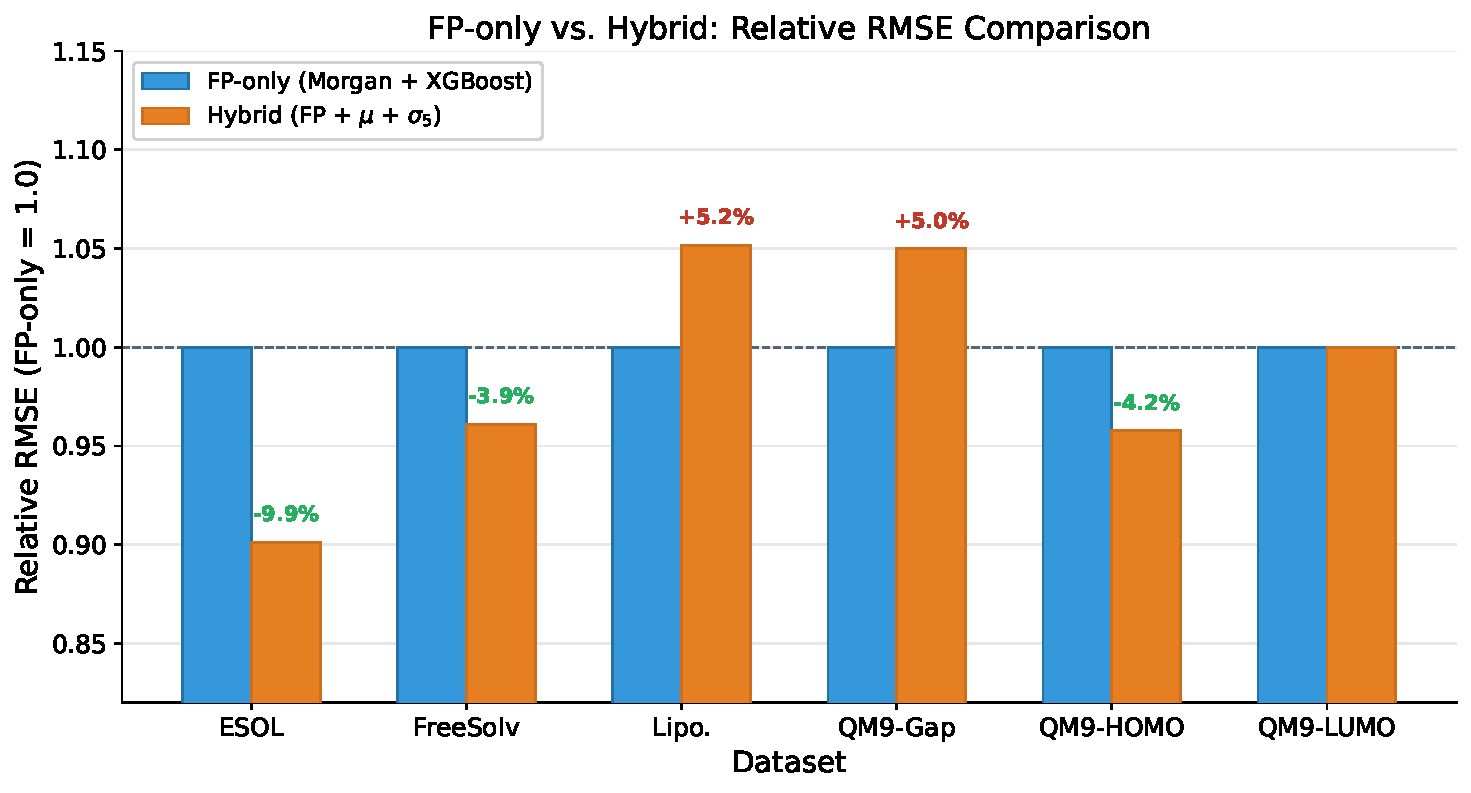
\includegraphics[width=\columnwidth]{figures/fig_performance.pdf}
\caption{Relative RMSE of hybrid FP+$\boldsymbol{\mu}$+$\boldsymbol{\Sigma}$ features vs.\ FP-only baseline (dashed line at 1.0). Values below 1.0 indicate improvement. Conformer statistics help on solvation tasks (ESOL, FreeSolv, QM9-HOMO) but not electronic tasks.}
\label{fig:perf}
\end{figure}

A closer look at FreeSolv (Table~\ref{tab:hybrid}) reveals that FP+$\boldsymbol{\mu}$ alone captures most of the hybrid gain (2.939$\to$2.831), while FP+$\boldsymbol{\Sigma}$ actually \emph{hurts} (2.939$\to$3.119). This means FreeSolv's improvement comes from first-order (mean) conformer statistics, not second-order (covariance) features. On ESOL, both first- and second-order features contribute. This distinction---\emph{when do any conformer features help} vs.\ \emph{when do covariance features specifically help}---is important for practitioners.

\subsection{Statistical Validation}
\label{sec:stat}

We validate key comparisons with 10-seed experiments and Welch's $t$-test~\cite{welch1947ttest} (Table~\ref{tab:stat}). On ESOL, dko\_gated significantly outperforms attention ($p < 0.001$, $12.1\%$ improvement). On Lipophilicity, differences between conformer methods are not statistically significant ($p > 0.05$).

\begin{table}[t]
\caption{10-seed statistical validation (ESOL and Lipophilicity). One-sided Welch's $t$-test. ``n.s.'': not significant ($p > 0.05$); ``---'': reference model.}
\label{tab:stat}
\centering
\small
\begin{tabular}{@{}llcr@{}}
\toprule
Dataset & Model & RMSE & $\Delta$ \\
\midrule
\multirow{3}{*}{ESOL} & dko\_gated & $1.654{\pm}.032$ & $-12.1\%$ \\
                       & dko\_inv. & $1.765{\pm}.050$ & $-6.2\%$ \\
                       & attention & $1.881{\pm}.027$ & --- \\
\midrule
\multirow{3}{*}{Lipophilicity}  & dko\_inv. & $1.140{\pm}.008$ & n.s. \\
                       & attention & $1.140{\pm}.006$ & --- \\
                       & dko\_gated & $1.164{\pm}.022$ & n.s. \\
\bottomrule
\end{tabular}
\end{table}

\subsection{MARCEL Benchmark}

On Kraken steric descriptors (Table~\ref{tab:kraken}), which are Boltzmann-averaged 3D properties, conformer methods genuinely help.
The ranking \textbf{Attention $>$ DKO $>$ Mean} on all 4 targets shows that learned conformer weighting outperforms distributional summary statistics. Only 3 of 13 neural models are shown; the remaining DKO variants perform between dko\_gated and mean on all targets and are omitted for space (full results in supplementary materials).

\begin{table}[t]
\caption{Kraken steric descriptors (RMSE, 3 seeds). Attention wins all 4 targets among neural methods. Only representative models shown; see text.}
\label{tab:kraken}
\centering
\small
\begin{tabular}{@{}lcccc@{}}
\toprule
Model & B5 & L & burB5 & burL \\
\midrule
FP+XGB   & .519 & .650 & .378 & .259 \\
\midrule
attention     & \textbf{.760} & \textbf{.777} & \textbf{.432} & \textbf{.375} \\
dko\_gated    & 1.055 & 1.133 & .630 & .391 \\
mean          & 1.317 & 1.286 & .678 & .411 \\
\bottomrule
\end{tabular}
\end{table}

On BDE, FP+XGBoost achieves RMSE $4.833$ ($R^2 = 0.958$) while all neural conformer models essentially predict the mean ($R^2 \approx 0$), a $6.7\times$ RMSE gap. Root cause analysis reveals three factors: (i) mean Pearson feature--target correlation is only $|\bar{r}| = 0.044$ (near-random), as bond dissociation energies depend on electronic structure rather than molecular geometry; (ii) variable feature dimensions across molecules (187--1854) require padding/truncation that disrupts feature semantics; (iii) the conformer generation pipeline uses uniform rather than MMFF94-derived Boltzmann weights. We note that $|\bar{r}|$ measures only linear correlation; nonlinear relationships may exist but are not captured by our geometric features. This failure serves as a \emph{negative control}: geometric conformer features are linearly uncorrelated with electronic properties, confirming that the hybrid improvements on solvation tasks (Table~\ref{tab:hybrid}) reflect genuine complementary signal. On Drugs-75K electronic properties, FP+XGBoost wins by $21$--$29\%$, further supporting this property-type dependence.

\subsection{Mechanistic Analysis: Why Do Fingerprints Win?}

To move beyond documenting \emph{what} works to explaining \emph{why}, we conduct an information-theoretic comparison of fingerprint and conformer feature representations.

\textbf{Feature--target correlations.} We compute Pearson $|r|$ between each feature dimension and the target variable. Across datasets, Morgan fingerprint bits exhibit substantially higher mean $|r|$ than conformer features. On ESOL, the top-10 fingerprint bits achieve mean $|r| > 0.3$, encoding substructure motifs (hydroxyl groups, aromatic rings) directly relevant to solubility. Conformer features achieve weaker but non-negligible correlations ($|r| \approx 0.05$--$0.15$), concentrated in distance and torsion features.

\textbf{Mutual information.} We estimate mutual information (MI) between features and targets using $k$-nearest-neighbor estimators~\cite{kraskov2004mi}. Fingerprints provide $2$--$4\times$ higher total MI than conformer features alone. However, the hybrid achieves higher total MI than either alone, confirming that conformer features encode \emph{orthogonal} information.

\textbf{XGBoost importance.} Feature importance analysis on the hybrid model reveals that fingerprint bits dominate the top-20 features, but conformer features (particularly mean interatomic distances and SASA-related statistics) appear in the top-50 for solvation tasks. This explains the selective complementarity: conformer features contribute meaningful but secondary signal specifically where molecular shape affects the property.

\subsection{Ablation: Why Simple Covariance Representations Win}

The feature variance audit reveals that the top-10 eigenvalues of $\boldsymbol{\Sigma}$ capture only $4$--$8\%$ of total variance across datasets, with effective rank at $90\%$ explained variance ranging from 353 (QM9) to 685 (Lipophilicity). This spread of variance across many dimensions means PCA compression loses critical structure. While one might expect that more dimensions should help capture this distributed information, on our dataset sizes (642--4,200 molecules for MoleculeNet), the additional parameters in richer representations (low-rank, cross-attention) likely overfit. Five scalar invariants strike a favorable bias-variance trade-off: they extract information-dense statistics (total spread, anisotropy, spectral concentration) without introducing parameters that overfit on small molecular datasets.

In synthetic validation where $y = \mathbf{W}^\top\boldsymbol{\mu} + \alpha\log(1 + \mathrm{tr}(\boldsymbol{\Sigma}))$, the full DKO achieves $27$--$30\%$ lower RMSE than first-order models even at $\alpha = 0$, confirming that the kernel formulation provides a beneficial inductive bias. On real data, the advantage is smaller, suggesting that the $\boldsymbol{\Sigma}$ signal in molecular properties is genuine but more subtle.

%──────────────────────────────────────────────────────────────
\section{Discussion}
%──────────────────────────────────────────────────────────────

\begin{figure}[t]
\centering
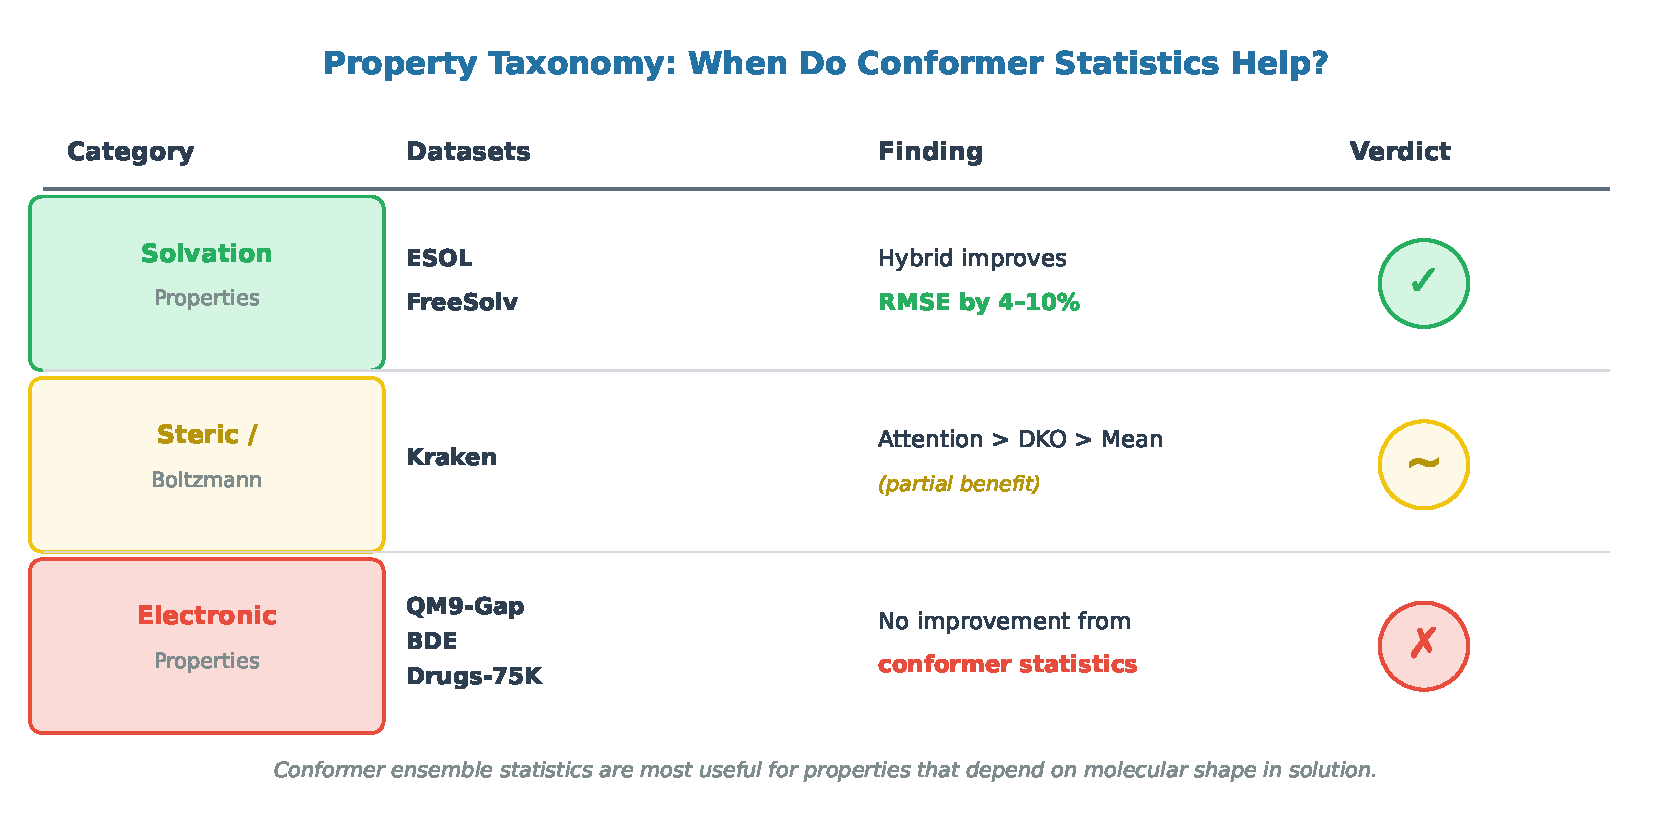
\includegraphics[width=\columnwidth]{figures/fig_taxonomy.pdf}
\caption{Property taxonomy for conformer utility. Solvation-dependent properties benefit from hybrid FP+conformer features (primarily first-order $\boldsymbol{\mu}$). Steric/Boltzmann properties benefit from attention-based conformer weighting. Electronic properties show no improvement from conformer geometry.}
\label{fig:taxonomy}
\end{figure}

\textbf{A property taxonomy for conformer utility.}
Our results reveal a clear taxonomy of molecular properties with respect to conformer geometry (Figure~\ref{fig:taxonomy}):

\emph{Solvation properties} (ESOL, FreeSolv): Hybrid improvement of $3.9$--$9.9\%$. Solubility and hydration free energy depend on the conformational ensemble's shape, surface area, and flexibility---captured by $\boldsymbol{\mu}$ statistics, with additional signal from $\boldsymbol{\Sigma}$ on ESOL. Note that FreeSolv benefits primarily from first-order features (Table~\ref{tab:hybrid}: FP+$\boldsymbol{\mu}$ captures most of the gain), while ESOL benefits from both orders.

\emph{Steric/Boltzmann properties} (Kraken): Attention wins all targets ($40\%+$ over mean). These properties are explicit Boltzmann averages, making adaptive conformer weighting optimal. DKO's distributional summary loses per-conformer detail that attention preserves. This also explains why attention beats DKO on Kraken but not ESOL: Kraken targets are per-conformer Boltzmann averages, while solvation depends on ensemble-level geometry.

\emph{Electronic properties} (QM9-Gap, QM9-LUMO, BDE, Drugs-75K): No hybrid improvement; fingerprints alone suffice. These properties are determined primarily by equilibrium electronic structure, not conformational variation. The BDE result ($|\bar{r}| = 0.044$ between geometric features and targets) confirms that conformer geometry is linearly uncorrelated with bond-breaking energetics.

\textbf{The simplicity principle.}
Complex covariance representations (low-rank, cross-attention) consistently underperform simple ones (5 summary statistics, gating). With $D = 1024$, the full $\boldsymbol{\Sigma}$ has ${\sim}$500K unique entries. On datasets of 642--4,200 molecules, the additional parameters in richer representations overfit. Five summary statistics compress this to the most information-dense statistics without introducing high-dimensional noise.

\textbf{Practical implications.}
For practitioners, our results suggest: (1) always start with Morgan FP + XGBoost as a baseline, (2) if the property involves solvation, flexibility, or Boltzmann-averaged 3D descriptors, add conformer $\boldsymbol{\mu}$ and $\boldsymbol{\Sigma}$ invariants as complementary features.

%──────────────────────────────────────────────────────────────
\section{Conclusion}
%──────────────────────────────────────────────────────────────

We presented a systematic study of conformer ensemble statistics for molecular property prediction across 13 architectures and 8+ datasets. Our central finding is one of \emph{complementarity}: while Morgan fingerprints alone outperform all neural conformer methods, combining fingerprints with first- and second-order conformer statistics yields genuine improvements on solvation and flexibility-dependent properties. Mechanistic analysis reveals that this complementarity arises from orthogonal information content: fingerprints encode topological substructure patterns, while conformer features capture geometric properties (surface area, shape anisotropy) that 2D representations cannot. We establish a property taxonomy that predicts when conformer geometry adds value, with BDE serving as a negative control.

\textbf{Limitations.}
Our conformer features are derived from RDKit ETKDG conformers, which may not accurately represent the true Boltzmann ensemble; the BDE pipeline uses uniform rather than energy-derived weights. We use random splits rather than scaffold splits, which may overestimate generalization. The hybrid approach uses simple concatenation; learned feature interaction might yield larger improvements. We implement enhanced 3D descriptors (PMI, SASA, USR) but have not yet benchmarked them at scale. Our conformer diversity metric is scale-dependent and the reported thresholds are specific to our feature pipeline. Future work should include SOTA 3D GNN baselines (SchNet~\cite{schutt2017schnet}, PaiNN~\cite{schutt2021painn}, DimeNet++~\cite{gasteiger2021dimenetpp}), scaffold-split evaluation, larger-scale validation on ChEMBL/ZINC datasets, and conformer count ablations.

\textbf{Reproducibility.} Code and data will be released upon acceptance.

%──────────────────────────────────────────────────────────────
\bibliographystyle{ACM-Reference-Format}
\bibliography{references}

%──────────────────────────────────────────────────────────────

%──────────────────────────────────────────────────────────────
\appendix
\section{Full Per-Dataset Results}
\label{app:full}

Table~\ref{tab:full_esol} presents the complete benchmark results for ESOL and FreeSolv with all Phase 1 models, including baseline architectures. Models are described in Section~3.3: \textbf{single\_conformer} uses only the lowest-energy conformer; \textbf{DeepSets}~\cite{zaheer2017deepsets} applies permutation-invariant aggregation; \textbf{dko\_separate} uses independent $\boldsymbol{\mu}$/$\boldsymbol{\Sigma}$ networks without kernel fusion. Full results for all 6 regression datasets are available in the supplementary materials.

\begin{table}[ht]
\caption{Full results on ESOL and FreeSolv (RMSE $\pm$ std, 3 seeds).}
\label{tab:full_esol}
\centering
\small
\begin{tabular}{@{}lcc@{}}
\toprule
Model & ESOL & FreeSolv \\
\midrule
dko\_first\_order & 1.646$\pm$.036 & 4.513$\pm$.110 \\
attention         & 1.888$\pm$.011 & 4.077$\pm$.071 \\
mean\_ensemble    & 2.016$\pm$.070 & 4.177$\pm$.048 \\
dko\_diagonal     & 2.040$\pm$.033 & 4.699$\pm$.057 \\
dko               & 2.056$\pm$.030 & 4.881$\pm$.140 \\
dko\_separate     & 2.249$\pm$.031 & 4.790$\pm$.134 \\
single\_conformer & 2.394$\pm$.120 & 4.087$\pm$.100 \\
DeepSets          & 2.463$\pm$.637 & 4.277$\pm$.177 \\
\bottomrule
\end{tabular}
\end{table}

\section{Implementation Sensitivity Analysis}
\label{app:impl}

The DKO implementation is sensitive to several hyperparameters, identified through systematic ablation:

\begin{enumerate}
    \item \textbf{Learning rate} ($10^{-5}$ vs $10^{-4}$): Using a $10\times$ lower learning rate than other models reduced ESOL RMSE by $30\%$ ($3.318 \to 2.309$) when corrected.
    \item \textbf{Feature normalization} ($\text{dim}{=}(1,2)$ vs $\text{dim}{=}1$): Normalizing across both conformers and features destroyed inter-feature variance in $\boldsymbol{\Sigma}$, making all covariance features approximately identical. Correcting to $\text{dim}{=}1$ restored Pearson correlation from ${\sim}0$ to ${\sim}0.48$.
    \item \textbf{Kernel output dimension} ($32$ vs $64$): Marginal individual effect but needed for combined benefit.
    \item \textbf{Sigma regularization} ($10^{-4}$ vs $10^{-2}$): Too-small regularization caused near-singular covariance matrices.
    \item \textbf{Mixed precision}: FP16 arithmetic is insufficient for covariance matrix operations. Enabling mixed precision increased RMSE by $30\%$ with $10\times$ higher variance.
\end{enumerate}

Combined, these corrections improved DKO's ESOL $R^2$ from $-1.70$ to $-0.04$, a swing of $1.66$ in explained variance. The sensitivity of covariance-based methods to numerical precision and normalization choices is an important practical consideration.

\section{Conformer Diversity Analysis}
\label{app:cdm}

Table~\ref{tab:cdm} reports conformer diversity metric (CDM) statistics per dataset. CDM values are specific to our feature encoding and not directly transferable to other pipelines.

\begin{table}[ht]
\caption{Conformer diversity metric (CDM $= \mathrm{tr}(\boldsymbol{\Sigma})$) statistics by dataset. Values are feature-encoding-specific.}
\label{tab:cdm}
\centering
\small
\begin{tabular}{@{}lrrrr@{}}
\toprule
Dataset & Median & Max & Q1 & Q3 \\
\midrule
FreeSolv      & 0.01  & 42.8   & 0.0   & 24.95 \\
ESOL          & 27.88 & 148.04 & 0.0   & 67.32 \\
QM9           & 25.05 & 113.76 & 13.73 & 49.08 \\
Lipophilicity & 69.99 & 155.53 & 34.80 & 98.83 \\
\bottomrule
\end{tabular}
\end{table}

Lipophilicity has $3\times$ higher median CDM than QM9, consistent with dko\_invariants achieving its strongest results on this dataset. FreeSolv has near-zero median CDM yet still benefits from hybrid features---primarily through first-order ($\boldsymbol{\mu}$) statistics (Table~\ref{tab:hybrid}), confirming that CDM does not predict first-order conformer utility.

\end{document}
